\documentclass{article}
\usepackage[utf8]{inputenc}
\usepackage[english]{babel}
\usepackage{amssymb}
\usepackage[letterpaper,top=2cm,bottom=2cm,left=3cm,right=3cm,marginparwidth=1.75cm]{geometry}
\usepackage{amsmath}
\usepackage{amsfonts}
\usepackage{amsthm}
\usepackage{graphicx}
\usepackage[colorlinks=true, allcolors=blue]{hyperref}
\usepackage{xcolor}
\usepackage{mathrsfs}
\usepackage{hyperref}
\usepackage{hyperref}

\newtheorem{definition}{Definition}
\newtheorem{proposition}{Proposition}
\newtheorem{remark}{Remark}
\newtheorem{lemma}{Lemma}
\newtheorem{corollary}{Corollary}
\newtheorem{theorem}{Theorem}
\title{Graph Rectifiability Exercises}
\author{Yutong Wu}
\date{May 2021}

\begin{document}
\maketitle

\section{Questions}
\begin{itemize}
    \item Day 5.26 1.12-1.16\\
    \item 1.2\\
$A_{\delta} = \{x : |x - y| \leq \delta for \ some \ y \ in \ A\}$\\
$A_{\delta + \delta'}$ is the $\delta$-neighborhood of $A_\delta$ with distance $\delta'$. Therefore we have:
$(A_\delta)_\delta' = \{x_\delta : |x_\delta - y_\delta| \leq \delta'\}$. It can also be interpreted as the  $\delta$-neighborhood of $A$ with distance $\delta + \delta'$. Thus we can rewrite it as: $(A_\delta)_\delta'= A_{\delta + \delta'} = \{x : |x - y| \leq \delta + \delta'\}$\\

\item 1.3\\
The set contained in the\\

\item 1.4\\
a)int(A) = the largest open set contained in A, cl(A) = the smallest closed set containing A. Cannot determined whether it is close or open.\\
b)open set. interior: $(0,1)$, closure:$[0,1]$.\\
c)closed set. interior: $(0,1)$, closure:$[0,1]$\\
d)closed set. interior: $(0,1)$, closure:$[0,1]$\\

\item 1.5\\
Firstly, middle three Cantor set is closed and bounded, which shows its compactness. Let $x, y \in C$ be distinct. Then, $x, y \in C_k$ for all $k \in \mathbb{N}$. Now, since x and y are distinct, we can find $N \in \mathbb{N}$ such that $\frac{1}{3^N} < |x - y|$. Hence, x and y belong to different intervals of $C_N$ . By the construction of the Cantor set, there must be at least one interval between x and y which does not belong to $C_N$ , and so does not belong to C. Select one such interval. Choosing any point z in this interval satisfies that z lies between x and y and $z \notin C$. Therefore, C is totally disconnected.

\item 1.6\\

\item 1.12\\
let $p(x) = f(x) + g(x)$ and $q(x) = f(x)g(x)$. Sine we know that both f(x) and g(x) are Lipschitz on [0,1], we can know that $|f(x) - f(y)| < C|x - y|$ and $|g(x) - g(y)| < C|x - y|$. To prove $|p(x) - p(y)| < C|x - y|$, we can rewrite it as $|(f(x)+g(x)) - (f(y)+g(y))| < C|x - y|$. Therefore we can see that the inequality is still hold, we can conclude that $p(x) = f(x) + g(x)$ is a Lipschitz function. Similar process for $q(x) = f(x)g(x)$. 
\item 1.13\\
Since $|f'(x)| \leq c$, By mean value theorem, $|\frac{f(y) - f(x)}{y - x}| = |f'(x)| \leq c$. Therefore we have $|f(y) - f(x)| \leq c|y-x|$, we can conclude that f(x) is Lipschitz.   
\item 1.14\\
By the definition of continuity, we have $
|f(x) - f(y)| < \delta$ and $|x-y| < \epsilon$ and $\delta.\epsilon > 0$. For all $\epsilon > 0, \forall \delta > 0$, s.t. if $|x - y| < \delta$ then $|f(x) - f(y)| < \delta$. If f is Lipschitz, and we have $\delta = \frac{\epsilon}{c}$ and c is the Lipschitz constant, if $|x-y|<\delta \rightarrow |x-y|<\frac{\epsilon}{c}$, we can get $|f(x) - f(y)| \leq C|x-y|\leq c*\frac{\epsilon}{c} = \epsilon$.
\item 1.15\\
(i) 1\\
(ii) $\phi$\\
(iii) [1,2]\\
\item 1.16\\
For any $x,y \in [0,2]$, we need to prove that $|f(x) - f(y)| \leq c|x - y|$ Since $f(x) = x^2$, we can rewrite the inequality into $|x^2 - y^2| \leq c|x - y| \rightarrow |(x+y)(x-y)| \leq c|x-y|\rightarrow|x+y| \leq c$. Since x and y are in [0,2], we can see that $|x + y| \leq 4$. Therefore, we can get $|f(x) - f(y)| \leq 4|x - y|$. Since $f(x) = x^2$, we know that $f^{-1}(x) = \sqrt{x}$. Since $\forall x,y \in [1,2]$, $\sqrt{x} < x$ and $\sqrt{y} < y$. We can conclude that $|f^{-1}(x) - f^{-1}(y)| \leq c|x-y|$. When expand the domain to $\mathbb{R}$, we cannot find such Lipschitz constant satisfy the inequality $|x+y| \leq c$, therefore $f(x)$ is only locally Lipschitz.\\

\item Day 5.26 1.18 1.23 1.24\\
\item 1.18\\
By 1.6, we know that $\mu(\cup_{i = 1}^\infty A_i) = \mu(A_1) + \sum_{i=1}^{\infty}(\mu(A_{i+1}) - \mu(A_{i}))=\lim_{i \rightarrow \infty}\mu(A_i)$. this expansion holds is because $A = \cup_{i = 1}^\infty A_i = A_1 \cup (A_2 \setminus A_3) \cup (A_3 \setminus A_2)...$ and $A_1 \subset A_2 \subset A_3...$ is an increasing sequence of Borel sets. In the given condition of question,  we know that $A = \cap_{i = 1}^\infty A_i = A_k / \cup_{i=1}^{k-1}A_i$ if $A_1...A_k$ intersect with each other. Or $A_1 ...A_k$ may have no intersection at all, which means $A = \emptyset$. For the second case, since empty set has zero measure and the diameter of $A_k$ tends to be zero as $k \rightarrow \infty$, we can prove that $\lim_{k\rightarrow \infty}\mu(A_k) = \mu(A)$.
For the first case, we can construct an increasing sequence ${A1 \setminus A_k}$ as ${A_k} $. decreasing.Then $\mu(\bigcap_{k=1}^{\infty}(A1 \setminus A_k)) = \mu(A_1 \setminus \bigcap_{k=1}^{\infty}A_i) = \mu(A_1) - \mu(A) = \lim_{k \rightarrow \infty}(A_1 \setminus A_k) = \lim_{k \rightarrow \infty}(\mu(A_1) - \mu(A_k)) = \mu(A_1) - \lim_{k \rightarrow \infty}\mu(A_k)$\\
since $\mu(A_1) < \infty$, we can say that $\mu(A) = \lim_{k \rightarrow \infty}\mu(A_k)$\\

\item 1.23\\
To prove the Egorov's theorem, we need to show that there exists a set A s.t. $\mu(D\setminus A) < \epsilon$ and ${f_k}$ is such that $\forall \delta >0$,there exists $k_\delta$.s.t.$k > k_\delta$then $| f_k(x) - f(x) | < \delta$.We first construct a increasing sequence of set A s.t. $A_{k,n} = \{x \in D: If \ l > k, \ then |f_l(x) - f(x)| < \frac{1}{n}\},\delta = \frac{1}{n}$ and the relation $A_{k,n} \subset A_{k+1,n}$ always hold. By the theorem, for $E_0 \supset E_1 \supset E_2 \supset E_3 \supset E_4...$, given that $\mu(E_0) < \infty$,we have $\lim_{i \rightarrow \infty}\mu(E_i) = \mu(\bigcap_{i=0}^{\infty}E_i)$ and $\mu(E_0) = \mu(\bigcup_{i=0}^{\infty}E_i)$

\item 1.24\\
The purpose of the question is actually to prove "the set E of points where $f(x) > 0$ has zero measure exists." Suppose $\epsilon > 0$ and $f(x) > \epsilon$, we have a set $E \subset D$.Since $\int_D f(x)d\mu = \int_E f(x)d\mu + \int_{D\setminus E}f(x)d\mu \geq \int_E \epsilon d\mu + 0 = \epsilon \mu(E) + 0$. Therefore we have $\epsilon \mu(E) \leq 0$, since $\epsilon > 0$, we have $\mu(E) = 0$. In a word, set E is the set of all points where f is greater than $\epsilon$ has measure zero. In other words, $f(x)\geq \epsilon$ $\mu$-almost everywhere. 


\item Day 6.3 2.1 2.2 2.4 2.5\\

\item 2.1
For a $\delta$-mesh grid, assume the center of each grid is exactly the center of each close ball with radii $\frac{\delta \sqrt{n}}{2}$. Let $N_\delta'(F)$ be the number of mesh grid cubes, then we have $N_{\frac{\delta \sqrt{n}}{2}} \leq N_\delta'(F) \rightarrow N
_{\delta \sqrt{n}} \leq N_{\frac{\delta \sqrt{n}}{2}} \leq N_\delta'(F) $. If a ball intersects a cube Q of side $\delta$, then to be precise, we can say that the ball is contained in at most four cube Qs, which in total $2^n$ cubes. Therefore we have $N'_\delta (F) \leq 2^n N_{\frac{\delta}{2}(F)}$. Combining the inequalities and dividing by $-\log \delta$, $\frac{\log N_{\delta \sqrt{n}}(F)}{-\log (\delta \sqrt{n}) + \log \sqrt{n}} \leq \frac{\log N'_\delta(F)}{-\log \delta} \leq \frac{\log 3^n + \log N_\delta(F)}{-\log \delta}$. So taking the lower limits as $\delta \rightarrow 0$, $\underline{\lim}_{\delta \rightarrow 0}\frac{\log N_\delta (F)}{-\log \delta} \leq \underline{\lim}_{\delta \rightarrow 0} \frac{\log N'_\delta(F)}{- \log \delta} \leq\underline{\lim}_{\delta \rightarrow 0}\frac{\log N_\delta (F)}{- \log \delta}$ with the other terms disappearing in the limit. Thus, the definition of 2.1-i works the same as 2.1-v. 
\item 2.2
If ${U_i}$ is a $\delta$-cover of F, then so is ${U_i \cap F}$. Taking images of these sets under f, we see that ${f(U_i \cap F)}$ is a $c\delta$-cover of $f(F)$, since by definition of Lipschitz mapping $|f(x) - f(y)| \leq c|x-y|$,  $|f(U_i \cap F)|\leq c|U_i \cap F|^\alpha\leq c|U_i|^\alpha\leq c\delta^\alpha$. Thus, we have $N_{c\delta}(F) \geq N_{c\delta^\alpha}(f(F))$ for all $\alpha > 0$, so $\frac{\log N_{c\delta}(f(F))}{-\log(c\delta)+\log c} \leq \frac{\log N_{\delta^\alpha}(F)}{-\alpha \log \delta}$. By taking lower and upper limits as $\delta \rightarrow 0$ gives the conclusion that $\underline{\dim}_B f(F) \leq \frac{1}{\alpha}\underline{\dim}_B F$ and $\overline{\dim}_B f(F) \leq \frac{1}{\alpha}\overline{\dim}_B F$
\item 2.4
The basic geometric observation here is that in construction of F shown in Figure 0.3, the $k^{th}$ stage of the construction consists of $4^k$ squares of side length and diameter $2^{-k}$. Thus, if $4^{-k} < \delta \leq 4^{-k+1}$, the $4^k$ squares of $E_k$ give a $\delta$ cover of F, so $N_\delta(F) \leq 4^k$, then $\bar{dim_m}F = \bar{\lim}_{\delta \rightarrow 0}\frac{\log N_\delta(F)}{-\log \delta} \leq \bar{\lim}_{k \rightarrow \infty} \frac{\log 4^k}{-\log 4^{-k+1}} = \frac{\log 4}{\log 4} = 1$. On the other hand, any square of side length $\delta$, where $4^{-k-1} \leq \delta < 4^{-k}$, can intersect at most two squares of $E_k$. There are $4^k$ squares in $E_k$ with side length $4^{-k}$, all containing points in F, so at least $4^k/2$ sets of side length $\delta$, or less are required to cover F. Hence $N_\delta(F) \geq 4^{k-\frac{1}{2}}$, so $\underline{\dim}_BF = \underline{\lim}_{\delta \rightarrow 0}\frac{\log N_\delta(F)}{-\log(\delta)} \geq \underline{\lim}_{\delta \rightarrow 0} \frac{\log 4^{k - 1/2}}{-\log 4^{-k - 1/2}} = 1$   
\item 2.5
If $3^{-k} < \delta \leq 3^{-k+1}$, then the $4^k$ level-k intervals of $E_k$ of length $3^{-k}$ provides a $\delta$-cover of F, so that $N_\delta(F) \leq 4^k$, where $N_\delta(F)$ is the least number of sets in a $\delta$-cover of F. From 2.3, $\overline{\dim}_B F = \overline{\lim}_{\delta \rightarrow 0} \frac{\log N_\delta (F)}{-\log \delta} \leq \overline{\lim}_{k \rightarrow \infty}\frac{\log 4^k}{-\log 3^{-k+1}} = \overline{\lim}_{k \rightarrow \infty}\frac{k \log 4}{(k-1)\log 3} = \frac{\log 4}{\log 3}$. On the other hand, any disjoint balls with radius $ 3^{-k-1}/2 < \delta \leq 3^{-k}/2$ and we have $4^k + 1$ disjoint balls in $E_k$, all containing points in curve with centres on curve. So at least $4^k +1$ disjoint balls of diameter $\delta$ or less are required to cover F. Hence, $N_\delta(F) \geq 4^k +1$,so $\underline{\dim}_B F = \underline{\lim}_{\delta \rightarrow 0}\frac{\log N_\delta (F)}{ - \log \delta} \geq \underline{\lim}_{k \rightarrow \infty}\frac{\log 4^k + 1}{-\log 1/2 * 3^{-k-1}} = \frac{\log 4 }{\log 3}$\\

\item 6.8 2.2 (revised) 3.7\\
2.2(revised)\\
3.7\\
\subtitle Approach a:\\
By the definition of Hausdorff dimension, we know that $H^1_{c\delta}() = 1$ which is just the length of the  interval. $H^1_{c\delta} (graph \ f) = \inf \sum_{i=1}^n |U_i|^1 \rightarrow \sum_{i=1}^n |f(U_i)|^1 \leq C\sum_{i=1}^n |U_i|$, where ${U_i}$ is the $c\delta$ cover of the graph f and for the $\sum_{i=1}^n |f(U_i)|^1$ is the $c\delta$ cover in the form of ${f(U_i)}$ where ${U_i}$ is the $\delta$-cover of the interval $[0,1]$. By taking infimum of $\sum_{i=1}^n |f(U_i)| \leq C\sum_{i=1}^n |U_i|$, we can find that $\inf (\sum_{i=1}^n |f(U_i)|\leq c*\sum_{i=1}^n |U_i|) \rightarrow H^1_{c\delta}(graph \ f) \leq c*H^1_\delta([0,1]) \rightarrow H^1_{c\delta}(graph \ f) \leq c$ as $\delta \rightarrow 0$. Therefore, $\dim_H graph \ f = 1$.\\
\subtitle Approach b:\\
Assuming $F(x) = (x,f(x))$, where $F: \ [0,1] \rightarrow graph \ f$, then we can conclude that $F$ is bi-Lipschitz since: 
\begin{align*}
&|F(x) - F(y)| = |(x,F(x)) - (y,f(y))|\\
&= \sqrt{(x-y)^2 + (F(x)-F(y))^2}\\
&\leq \sqrt{(x-y)^2 + c^2(x-y)^2}\\
&\leq (1+c)^2|x-y|
\end{align*}
Therefore, we have $|x-y|\leq |F(x) - F(y)|\leq(1+c)^2|x-y|$. Since $F$ is a bi-Lipschitz function, by proposition 3.2.1, we can conclude that $\dim_H graph \ f = \dim_H [0,1] = 1$. 

\item Day 6.10 5.2 5.8\\ 
\item 5.2\\
Since $0<c_1<f'(x)<c_2$, we can rewrite this sequence of inequality as $0<c_1<\frac{|f(x)-f(y)|}{|x-y|}<c_2 \rightarrow 0 < c_1|x-y|<|f(x)-f(y)|<c_2|x-y|$. Thus, we can assume that function f is bi-Lipschitz when x and y are small. As function f is bi-Lipschitz, $\dim_H F = \dim_H f(F)$ and $H^1(f(F)) = c_2H^1(F)$ by proposition 3.3 b and scaling property of the Hausdorff measure. To show that the lower and upper density of set $F$ and $f(F)$ are equal, we need to show that $H^1(f(F) \cap B(f(x),r)) = H^1(F\cap B(x,r))$. Since \[c_1H^1(F)\leq H^1(f(F))\leq c_2H^1(F)\] and the definition of the density is \[D(F,x) = \lim_{r \to 0}\inf{\frac{H^s(F \cap B(x,r))}{(2r)^s}}\], we can rewrite the density equality into this form:
\begin{align*}
&\lim_{r \to 0}\inf{\frac{H^s(f(F) \cap B(f(x),r))}{(2r)^s}}\\
&=\lim_{r \to 0}\inf{\frac{H^s(f(F) \cap B(f(x),c_1r))}{(2c_1r)^s}}\\
&=\lim_{r \to 0}\inf{\frac{H^s(f(F) \cap B(f(x),c_1r))}{c_1^s(2r)^s}}\\
&\geq \lim_{r \to 0}\inf{\frac{c_1^s H^s(F \cap B(x,r))}{c_1^s(2r)^s}}\\
&\geq \lim_{r \to 0}\inf{\frac{ H^s(F \cap B(x,r))}{(2r)^s}}
\end{align*}
For right side:
\begin{align*}
&\lim_{r \to 0}\inf{\frac{H^s(f(F) \cap B(f(x),r))}{(2r)^s}}\\
&\lim_{r \to 0}\inf{\frac{H^s(f(F) \cap B(f(x),c_2r))}{(2c_2r)^s}}\\
&=\lim_{r \to 0}\inf{\frac{H^s(f(F) \cap B(f(x),c_2r))}{c_2^s(2r)^s}}\\
&\leq \lim_{r \to 0}\inf{\frac{c_2^s H^s(F \cap B(x,r))}{c_2^s(2r)^s}}\\
&\leq \lim_{r \to 0}\inf{\frac{ H^s(F \cap B(x,r))}{(2r)^s}}
\end{align*}
Finally we have \[\lim_{r \to 0}\inf{\frac{ H^s(F \cap B(x,r))}{(2r)^s}} \leq \lim_{r \to 0}\inf{\frac{H^s(f(F) \cap B(f(x),r))}{(2r)^s}} \geq \lim_{r \to 0}\inf{\frac{ H^s(F \cap B(x,r))}{(2r)^s}}\]. We can conclude that the density of F is the same as f(F).
\item 5.8\\
If we know that $F_k$ are regular 1-sets, all of them consists of a curve like portion and a portion with $H^1$ measure zero. Since $F = \bigcup_{k=1}^{\infty} F_k$, we can conclude that F also consists of a curve-like portion and a portion with $H^1$-measure equals 0. If each $F_k$ is curve free, by definition $H^1(C \cap F_k) = 0$ where C is a rectifiable curve. Then, $0 \leq H^1(C \cap \bigcup_{k=1}^\infty F_k) = H^1(\bigcup_{k=1}^\infty(C \cap F_k)) \leq \sum_{k=1}^\infty H^1(C \cap F_k) = 0$. s.t. F is curve free. By Theorem 2.1.3 b., F is irregular. \\

\subsubsection{doubling measure}
\begin{proof}
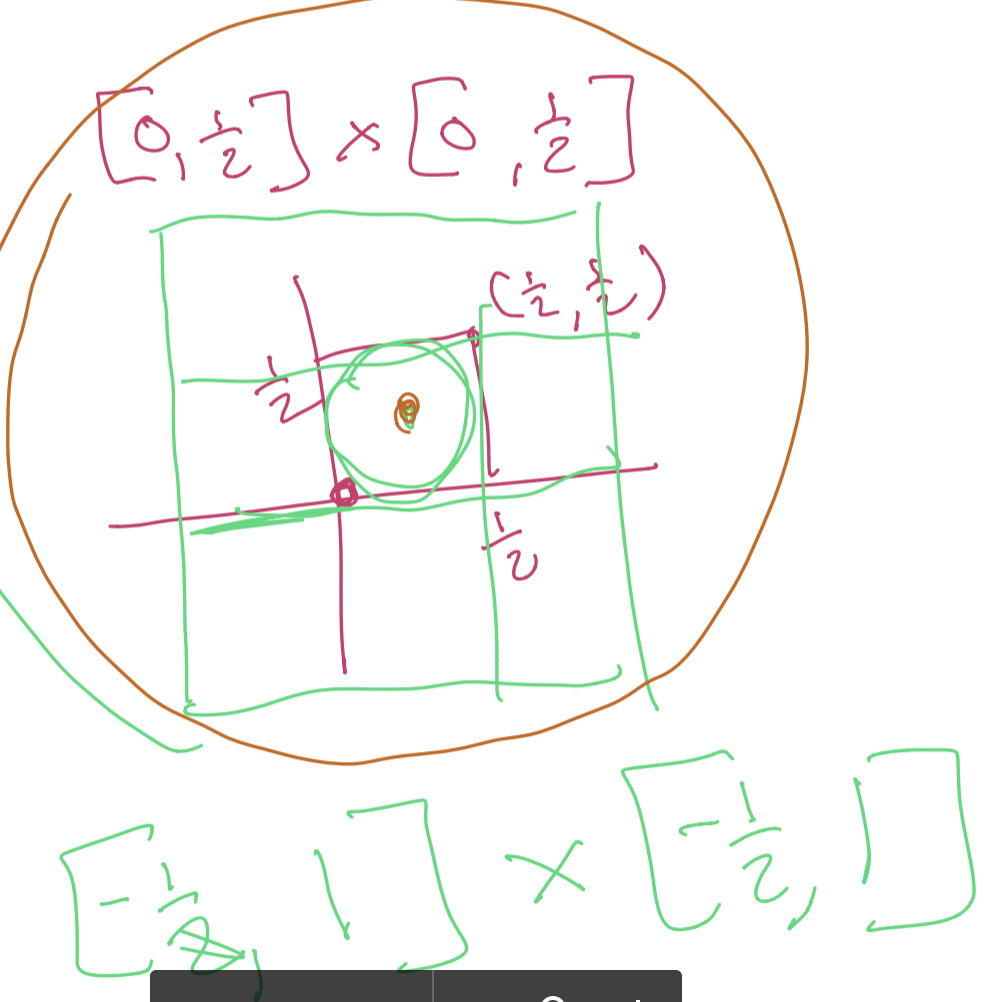
\includegraphics[width=8cm, height=8cm]{doubling measure.png}\\
Since we know that $\mu(B(x,2r))\leq K(\mu(B(x,r)))$, we can see that the inner ball $B(x,r)$ has radius r equals $1/4$ which is the half of the side length of Q and the outer ball $B(x,R)$has radius equals to $\frac{3\sqrt{2}}{2}$ which is the half of the diameter of the 3Q. From here we can find that the radius of the outer ball is also larger than the ball with radius 2r which is $1/2$ (not shown in the picture). Thus we can say that there exists a K such that $\mu(B(x,2r))\leq K(\mu(B(x,r)))$. Since t $\mu(B(x,r)) \le \mu(Q)$ and there exists K that enlarge $\mu(B(x,r))$ to be greater than $\mu(3Q)$, we can say that there also exists K that satisfy $\mu(3Q) \leq K\mu(Q)$.\\
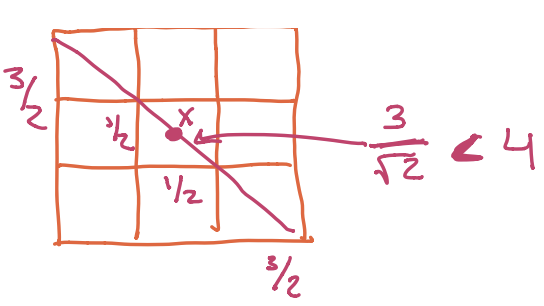
\includegraphics[width=15cm, height=8cm]{dm2.png}\\
Let $Q = [0,\frac{1}{2}]*[0,\frac{1}{2}]$ and $3Q = [-\frac{1}{2},1]*[-\frac{1}{2},1]$, x be the center of $Q(1/4,1/4) = x$.Then $B(x, 1/4) \subset Q \subset 3Q \subset B(x,4)$and $4 = 2^4 * 1/4 = 16*1/4$, which means that we need to double the radius of B(x,1/4) 4 times to get B(x,4).From doubling property of measure that means:
\begin{align*}
&\mu(B(x,4)) \leq K\mu(B(x,2))\\
&\leq K(K\mu(B(x,1))\\
&\leq K^2(K\mu(B(x,1)))\\
&\leq K^2(K\mu(B(x,1/2)))\\
&\leq K^3(K\mu(B(x,1/4)))
\end{align*}
Therefore we have \[*\mu(B(x,4))\leq K^4\mu(B(x,1/4))\].
Now since $3Q\subset B(x,4)$, $\mu(3Q)\leq \mu(B(x,4))\rightarrow Q \subset B(x,1/4)\rightarrow \mu(Q) \geq \mu(B(x,1/4))$. By using *, we can get:
\begin{align*}
&\mu(Q) \geq \mu(B(x,1/4))\\
&\geq K^{-4}\mu(B(x,4))\\
&\geq K^{-4}\mu(3Q)
\end{align*}
In particular, $K^4\mu(Q)\geq\mu(3Q)$\\
\end{proof}


\end{itemize}

\subsection{Research Questions} 
\subsection{Definitions}
we define the bad cone using dyadic cube with following two definitions:
\begin{align}
   \mathcal{C}^{1}_\mathcal{B}(Q,V,\alpha) = \bigcup_{x\in Q}\mathcal{C}_\mathcal{B}(x,V,\alpha)\\
    \mathcal{C}^{2}_\mathcal{B}(Q,V,\alpha) = \bigcap_{x\in Q}\mathcal{C}_\mathcal{B}(x,V,\alpha)
\end{align}
To be more specific about the content included in the bad cones under dyadic cube regime, we further define it based on two different situations of the intersection of the bad cone edge and the cubes. In the following definition, R denotes the dyadic cubes of same side length of Q:
\begin{align}
   \mathcal{C}^{1,1}_\mathcal{B}(Q,V,\alpha) = \{R|R\cap(\bigcup_{x\in Q}\mathcal{C}_\mathcal{B}(x,V,\alpha))\}\\
    \mathcal{C}^{1,2}_\mathcal{B}(Q,V,\alpha) = \{R|R\subset(\bigcup_{x\in Q}\mathcal{C}_\mathcal{B}(x,V,\alpha))\}
\end{align}
\section{Condition for rectifiability}

\begin{theorem}[Geometric Lemma] Let $F\subset \rr^2$, and fix $V\in G(1,2)$ and $\alpha\in(0,1)$.  If 
	\[F\cap \mathcal{C}_\mathcal{B}(x,V, \alpha)=\emptyset\text{ for all }x\in F\]
	then $F$ is contained in an $1$-Lipschitz graphs.  In particular, $F\subset\Gamma$ where $\Gamma$ is a Lipschitz graph with respect to $V$ and the Lipschitz constant corresponding to $\Gamma$ is at most $1+1/(1-\alpha^2)^{1/2}$.
	\label{thm:geometric_lemma}
\end{theorem}

Applying the second definition of bad cone, if we can show $\mathcal{C}^2_\mathcal{B}(Q,V,\alpha)$ converge to $\mathcal{C}^2_\mathcal{B}(x,V,\alpha)$ as we generate more generations of children of cube, i.e.\[\mathcal{C}^2_\mathcal{B}(Q,V,\alpha)\to \mathcal{C}^2_\mathcal{B}(x,V,\alpha),\lim_{K\to 0}Q \to x\]


\begin{lemma}
Let $\mu$ be a Radon measure on $\rr^2$, and fix $V\in G(1,2)$ and $\alpha\in(0,1)$.  Suppose $E\subset\rr^2$ such that for every $x\in E$ and for every dyadic cube $Q$ containing $x$, \[\mu(\mathcal{C}_\mathcal{B}^2(Q,V,\alpha))=0.\] Then $E$ is contained $\mu$- almost everywhere in a $1$-Lipschitz graph.
\end{lemma}

\textcolor{red}{Note: $V\in G(1,2)$ is a formal way to say $V$ is a line in $\rr^2$ going through the origin.  The $G$ stands for Grassmanian.}

Explanation (replaced with formal proof later): \\ The direction of m-dimensional linear plane V and $\alpha$ is fixed when constructing bad cones(i.e. Each plane $V_i$ of each sets of bad cones are parallel to each other and the aperture for each cone is fixed). As we generate more generation of children cubes and try to construct the new bad cones $\mathcal{C}_{\mathcal{B}_i}$with respect to new plane $V_i$, the new planes are approaching the corner point and the side of original cube depending on the direction of the plane we use. As new plane $V_i$ approaches the margin of the original cube, we can see that the bad cones $\mathcal{C}_{\mathcal{B}_i}$ with respect to it approaches to be the bad cones centered at points inside the original cube and finally to be the ones centered at the points on the edges of the original cube. More specifically, small $\alpha$ is preferred since it allows the new bad cones $\mathcal{C}_{\mathcal{B}_i}$ to be the most efficiently capture the content of the old bad cones.\\
If we pick $y \in \mathcal{C}_\mathcal{B}(x,V,\alpha)$ show that there is sufficiently small $Q_s$ so that \[y\in \mathcal{C}^2_\mathcal{B}(Q_s,V,\alpha)\]\\
Construct ball $B(x,|x-y|)$. Given that $x\in Q$ and $Q \to x$, if $B(x,|x-y|) \cap Q \neq \O$ and $Q \notin B(x,|x-y|)$, we can say that $y \in Q_s$ s.t.$Q_s \in Q$.\\

\begin{lemma}[Doubling condition for cubes]
Let $\mu$ be a Radon measure on $\mathbb{R}^2$.  Suppose that for all $r>0$, $\mu(B(x, 2r))\le D_1\mu(B(x,r))$.  If $Q_k$ be a dyadic cube of side length $k$ such that $x\in Q_k$ then $\mu(4Q)\le D_2\mu(2Q).$\\
\end{lemma}

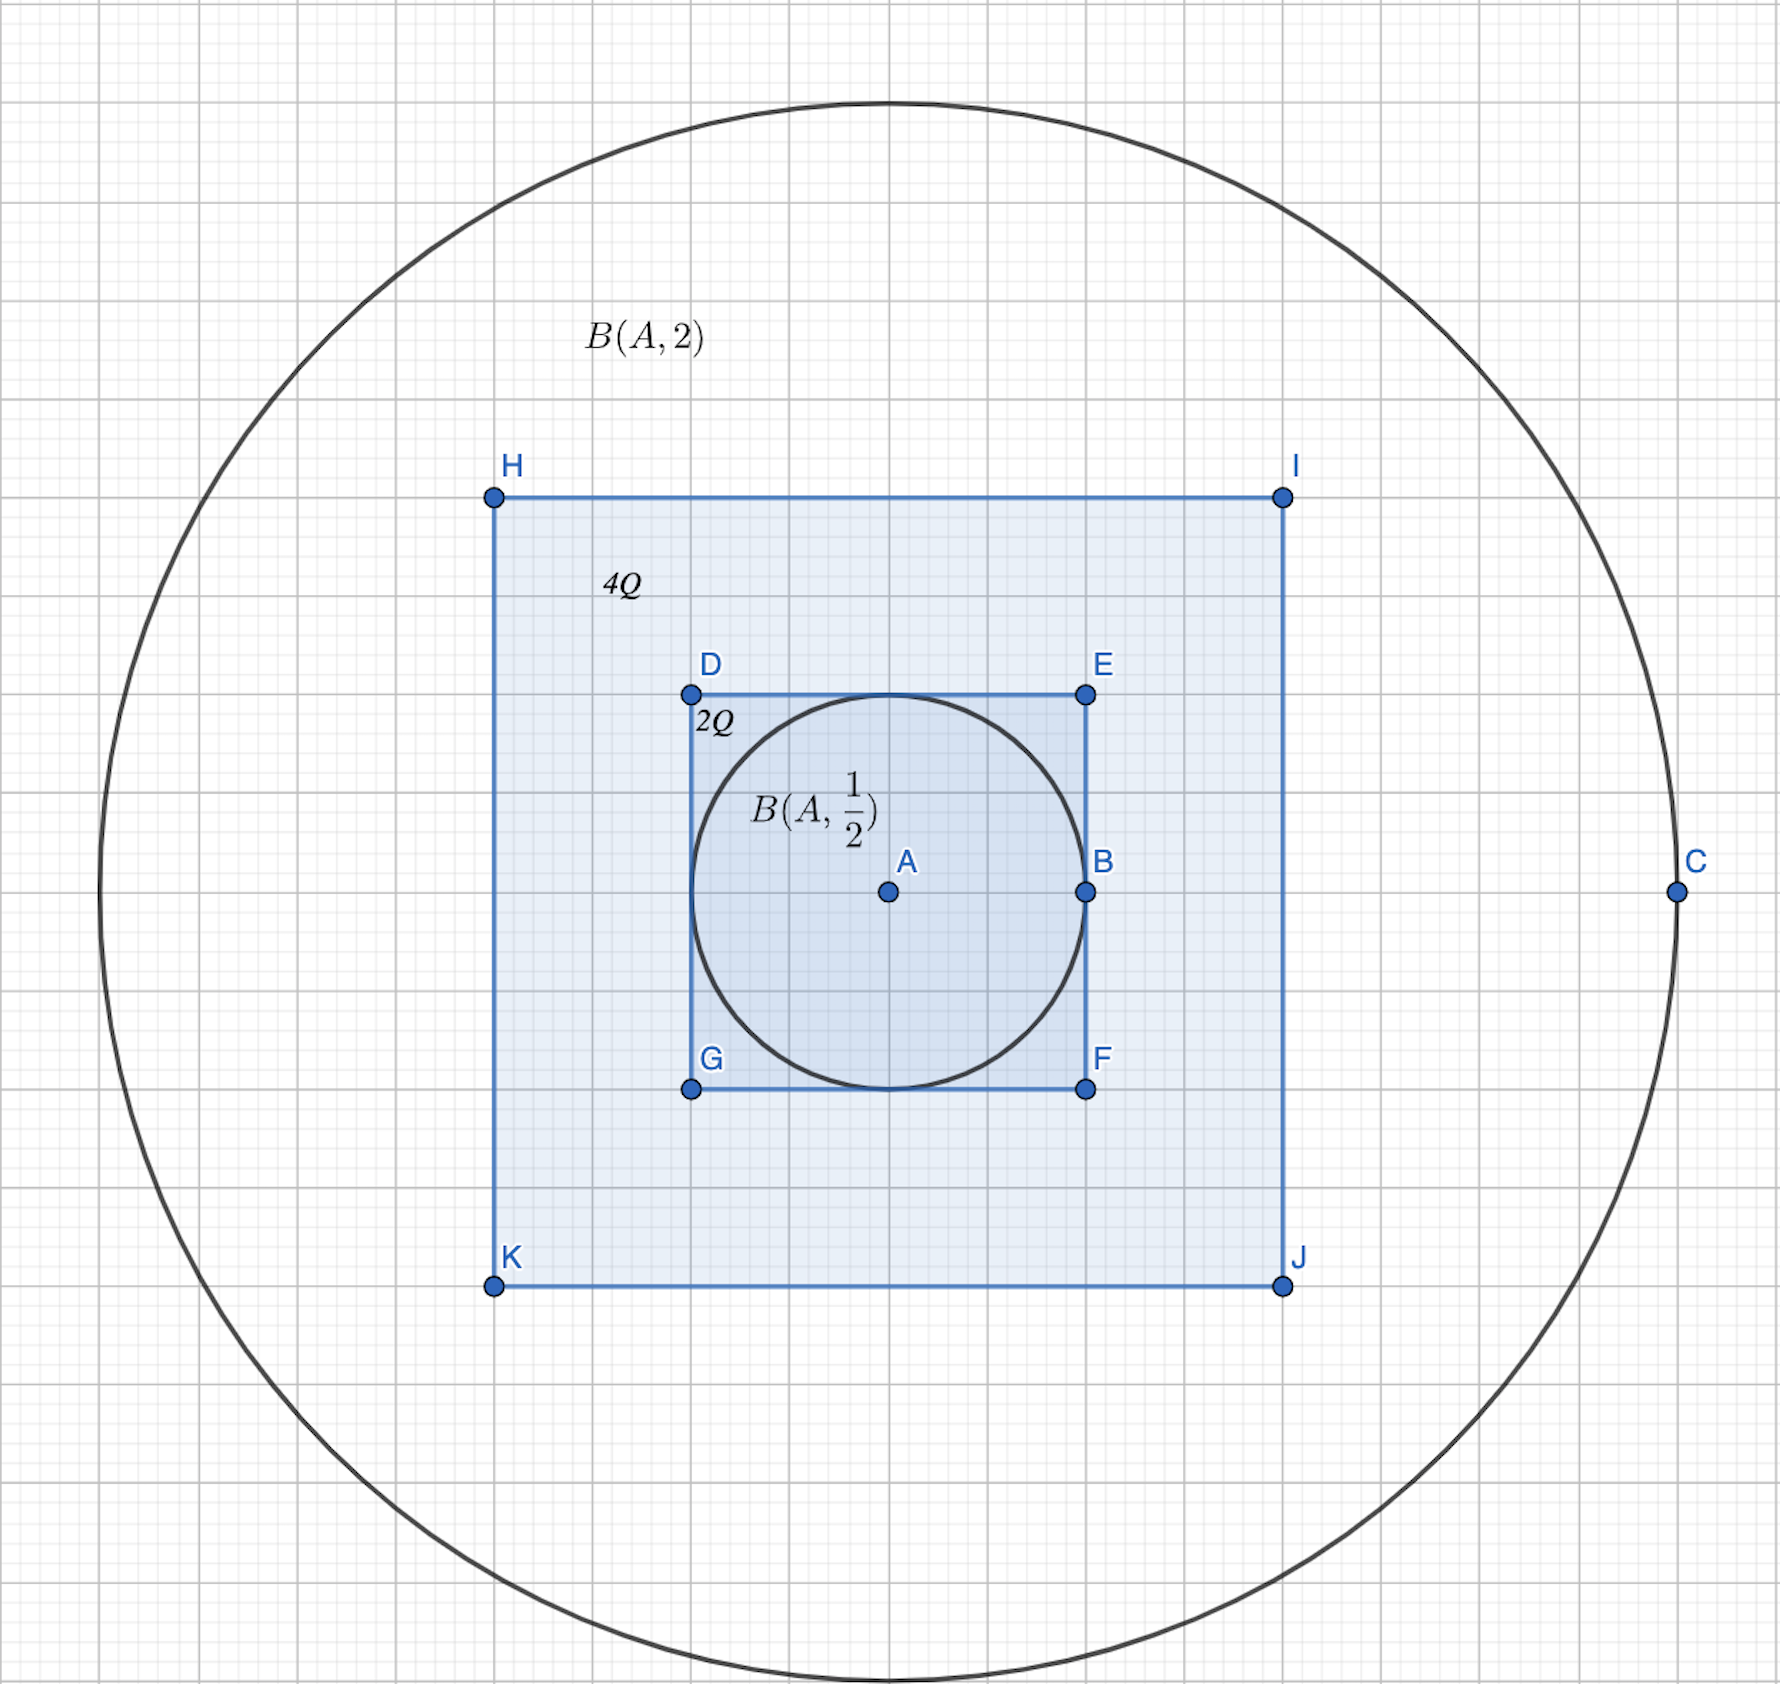
\includegraphics[width = 3in, height = 3in]{Screen Shot 2021-06-22 at 10.18.14 AM.png}\\
\begin{proof}\\
Let $Q = [0,\frac{1}{2}]*[0,\frac{1}{2}]$,$2Q = [-\frac{1}{2},\frac{1}{2}]*[-\frac{1}{2},\frac{1}{2}]$ and $4Q = [-1,1]*[-1,1]$, x be the center of $Q(0,0) = x$.Then $B(x, 1/2) \subset 2Q \subset 4Q \subset B(x,2)$and $2 = 2^2 * 1/2 = 4*1/2$, which means that we need to double the radius of B(x,1/2) twice to get B(x,4).From doubling property of measure that means:
\begin{align*}
&\mu(B(x,2)) \leq K\mu(B(x,1))\\
&\leq K\mu(B(x,1))\\
&\leq K(K\mu(B(x,1/2)))
\end{align*}
Therefore we have \[*\mu(B(x,2))\leq K^2\mu(B(x,1/2))\].
Now since $4Q\subset B(x,2)$, $\mu(4Q)\leq \mu(B(x,2))\rightarrow B(0,1/2) \subset 2Q\rightarrow \mu(2Q) \geq \mu(B(x,1/4))$. By using *, we can get:
\begin{align*}
&\mu(2Q) \geq \mu(B(x,1/2))\\
&\geq K^{-2}\mu(B(x,2))\\
&\geq K^{-2}\mu(4Q)
\end{align*}
In particular, $K^2\mu(2Q)\geq\mu(4Q)$
\end{proof}
\begin{lemma}\label{lemma:CBQ2carried}
A nontrivial measure on a metric space X is said to be doubling if the measure of any ball is finite and approximately the measure of its double, or more precisely, if there is a constant $K > 0$ such that for all $x \in X$ and $r > 0$. In this case, we say $\mu$ is K-doubling.
    \begin{equation}\label{muB2=0}
         0<\mu (B(x,2r))\leq K\mu (B(x,r))<\infty
    \end{equation}
    Then $E$ is contained $\mu$-almost everywhere in a $K$-Lipschitz graph.
\end{lemma}
We would like to expand this doubling property of measure to the dyadic cube regime. Without loss of generality, let $Q$ be a cube with $2^{-k}$ as side length and 3Q to be the dilation of $Q$ with side length $3*2^{-k}$ and 5Q to be a further dilation with side length $5*2^{-k}$. There exists a ball $B(p,2^{-k-1})$ with center $p$ such that $p$ is a random point and $p \in Q$. Since we need to prove that $\exists m$ s.t. \[\mu(5Q) \leq K^m \mu(3Q)\]
\begin{proof}
We can firstly construct a larger ball $B_l$ that enclose $5Q$. To construct such ball, we need to make sure its radius is greater than the furthest distance from the center of $B(p,2^{-k-1})$ to the boundary of $5Q$. The furthest distance exists if and only if p falls on one of the corner of the cube $Q$ like the figure shown. Let $x \in Q$ such that for all $r > 0$. we have doubling measure \[\mu(B(x,2r))\leq K\mu(B(x,r))\] According to the figure, we have here try to estimate the distance between a point $S\in B(x, 2^{-k-1})$ and the center point of the cube q. Then say $S$ is close enough to $q$ so that it must be contained in $3Q$ 
\begin{figure}
    \centering
    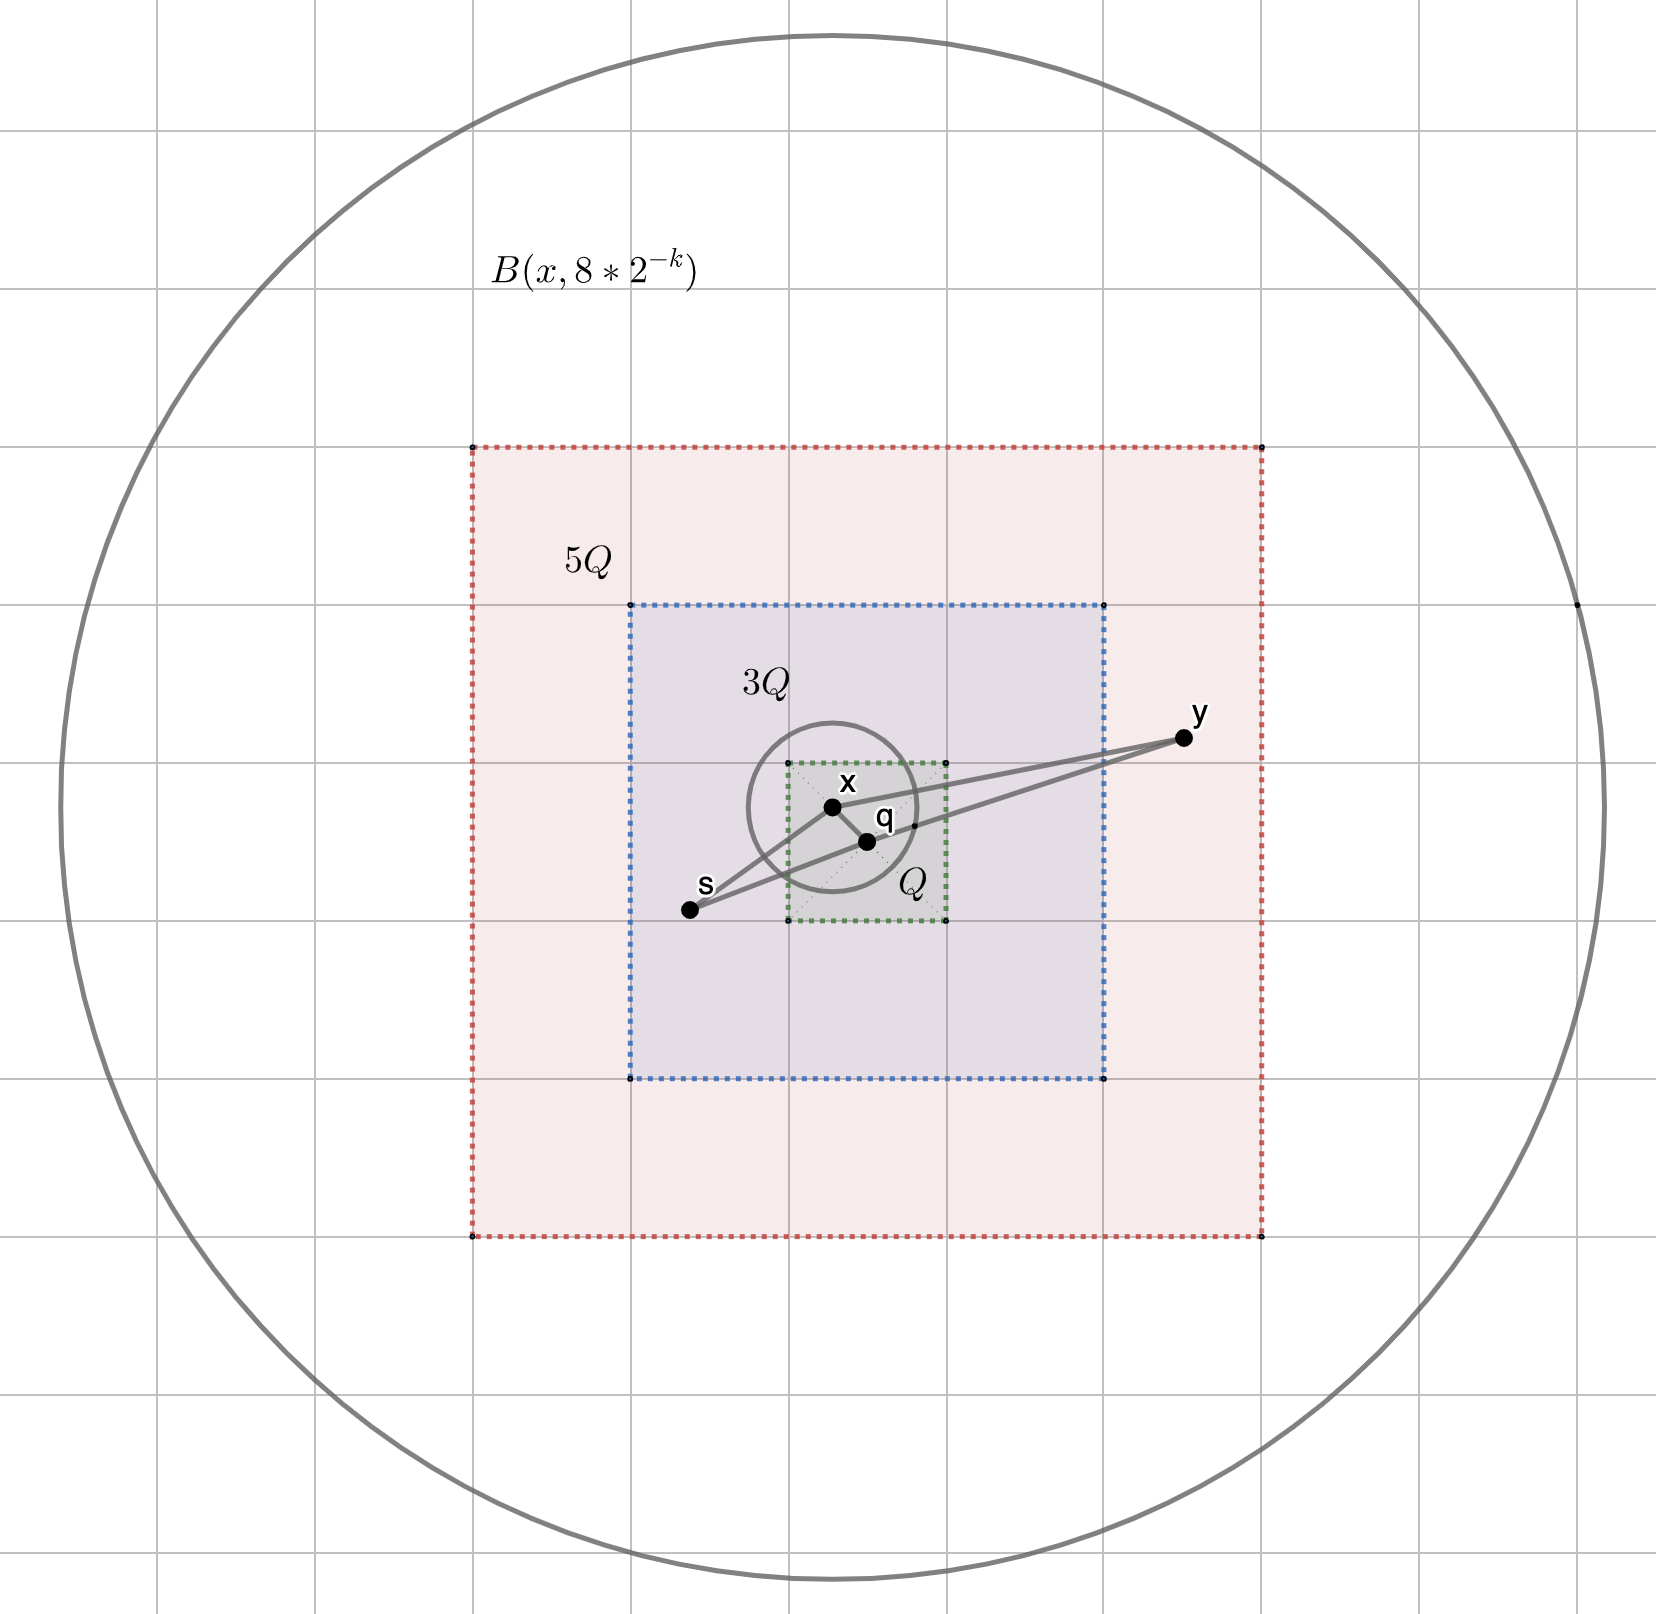
\includegraphics[width = 3in, height = 3in]{dm.png}
    \caption{doubling measure}
    \label{fig:my_label}
\end{figure}
\begin{equation*}
    \begin{aligned}
        |x - S| & \leq |x - q| + |q - S| \\
        & \leq \frac{diam(Q)}{2} + \frac{diam(3Q)}{2} \\
        & =\sqrt{2}*2^{-(k-1)}/2 + 3\sqrt{2}*2^{-(k-1)}/2 \\
        & =2\sqrt{2}*2^{-k} \\
        & =2^{-k + \frac{3}{2}}
    \end{aligned}
\end{equation*}
Since $B(x , 2^{-k-1})$ have radius $2^{-k-1} < 2^{-k + 3/2}$, we obtain that $B(x,2^{-(k-1)}) \subset 3Q$. Additionally, if $y \in 5Q$, we have:
\begin{equation*}
    \begin{aligned}
        |y - x| & \leq |y - q| + |q - x| \\
        & \leq \frac{diam(5Q)}{2} + \frac{diam(Q)}{2} \\
        & =5\sqrt{2}*2^{-k}/2 + \sqrt{2}*2^{-k}/2 \\
        & =3\sqrt{2}*2^{-k} \\
        & <2^3*2^{-k}
\end{aligned}
\end{equation*}
Therefore, we have $5Q \subset B(x,2^3*2^{-k})$ and $B(x,2^{-k-1}) \subset 3Q \subset 5Q \subset B_l(x, 2^3*2^{-k})$
\begin{equation*}
    \begin{aligned}
    \mu(B(x,2^3*2^{-k})) & \leq K\mu(B(x,2^2*2^{-k}))\\
    & \leq K(K\mu(B(x,2*2^{-k}))) \\
    & \leq K^2(K\mu(B(x,2^0*2^{-k}))) \\
    & \leq K^3(K\mu(B(x,2^{-1}*2^{-k}))) \\
    & \leq K^4\mu(B(x,2^{-k-1}))
\end{aligned} 
\end{equation*}
Thus we get
\begin{equation}
    \mu(B(x,2^3*2^{-k})) \leq K^4\mu(B(x,2^{-k-1}))
\end{equation}
Now since $5Q\subset B(x,2^3*2^{-k})$, $\mu(5Q)\leq \mu(B(x,2^3*2^{-k}))\rightarrow B(x,2^{-k-1}) \subset 3Q\rightarrow \mu(3Q) \geq \mu(B(x,2^{-k-1}))$. By using (7), we can get:\\
\begin{equation*}
    \begin{aligned}
        \mu(3Q) & \geq \mu(B(x,2^{-(k-1)})) \\
        & \geq K^{-4}\mu(B(x,2^3*2^{-(k-1)})) \\
        & \geq K^{-4}\mu(5Q)
    \end{aligned}
\end{equation*}
In particular, $K^4\mu(3Q)\geq\mu(5Q)$
\end{proof}

\begin{lemma}
For $\alpha_1,\alpha_2\in(0,1)$, $\alpha_1 > \alpha_2$, there is a m-plane in $\mathbb{R}^n$ such that for a cube Q with side length $2^{-|k|}$, and a cube R with the same side length as $Q$, how far of R away from $Q$ needs to be guaranteed such that \[R\in C^{1,1}_B(Q,V,\alpha_1), R\in C^{1,2}_B(Q,V,\alpha_2)\]\\
\end{lemma}

\begin{proof}
By assumption, there are some $x\in R$ and $x \in C^{1,1}_B$ such that there exists $q \in Q$ such that $y \in C_B(q,V,\alpha_1)$. Then $dist(x-q,V)> \alpha _1 |x - q|$. Now assume that $|x - q| = s*2^{|k|}$. Then to satisfy (1), for any $y \in R$, there exists $q' \in Q$ such that $y \in C_B(q', V, \alpha)$.Now we have $|x - y| \leq \sqrt{n}2^{|-k|}$, $|q - q'|\leq \sqrt{n}2^{-k}$. Since 
\begin{equation*}
\begin{aligned}
    dist(y - q', V) &\geq dist(x - q, V) - |q' - q| - |x - y| \\
    & > \alpha_1|x - q| - \sqrt{n}2^{-|k|+1} \\
    & = \alpha_1|s2^{-|k|}| - \sqrt{n}2^{-|k| + 1}
\end{aligned}
\end{equation*}
\begin{figure}
    \centering
    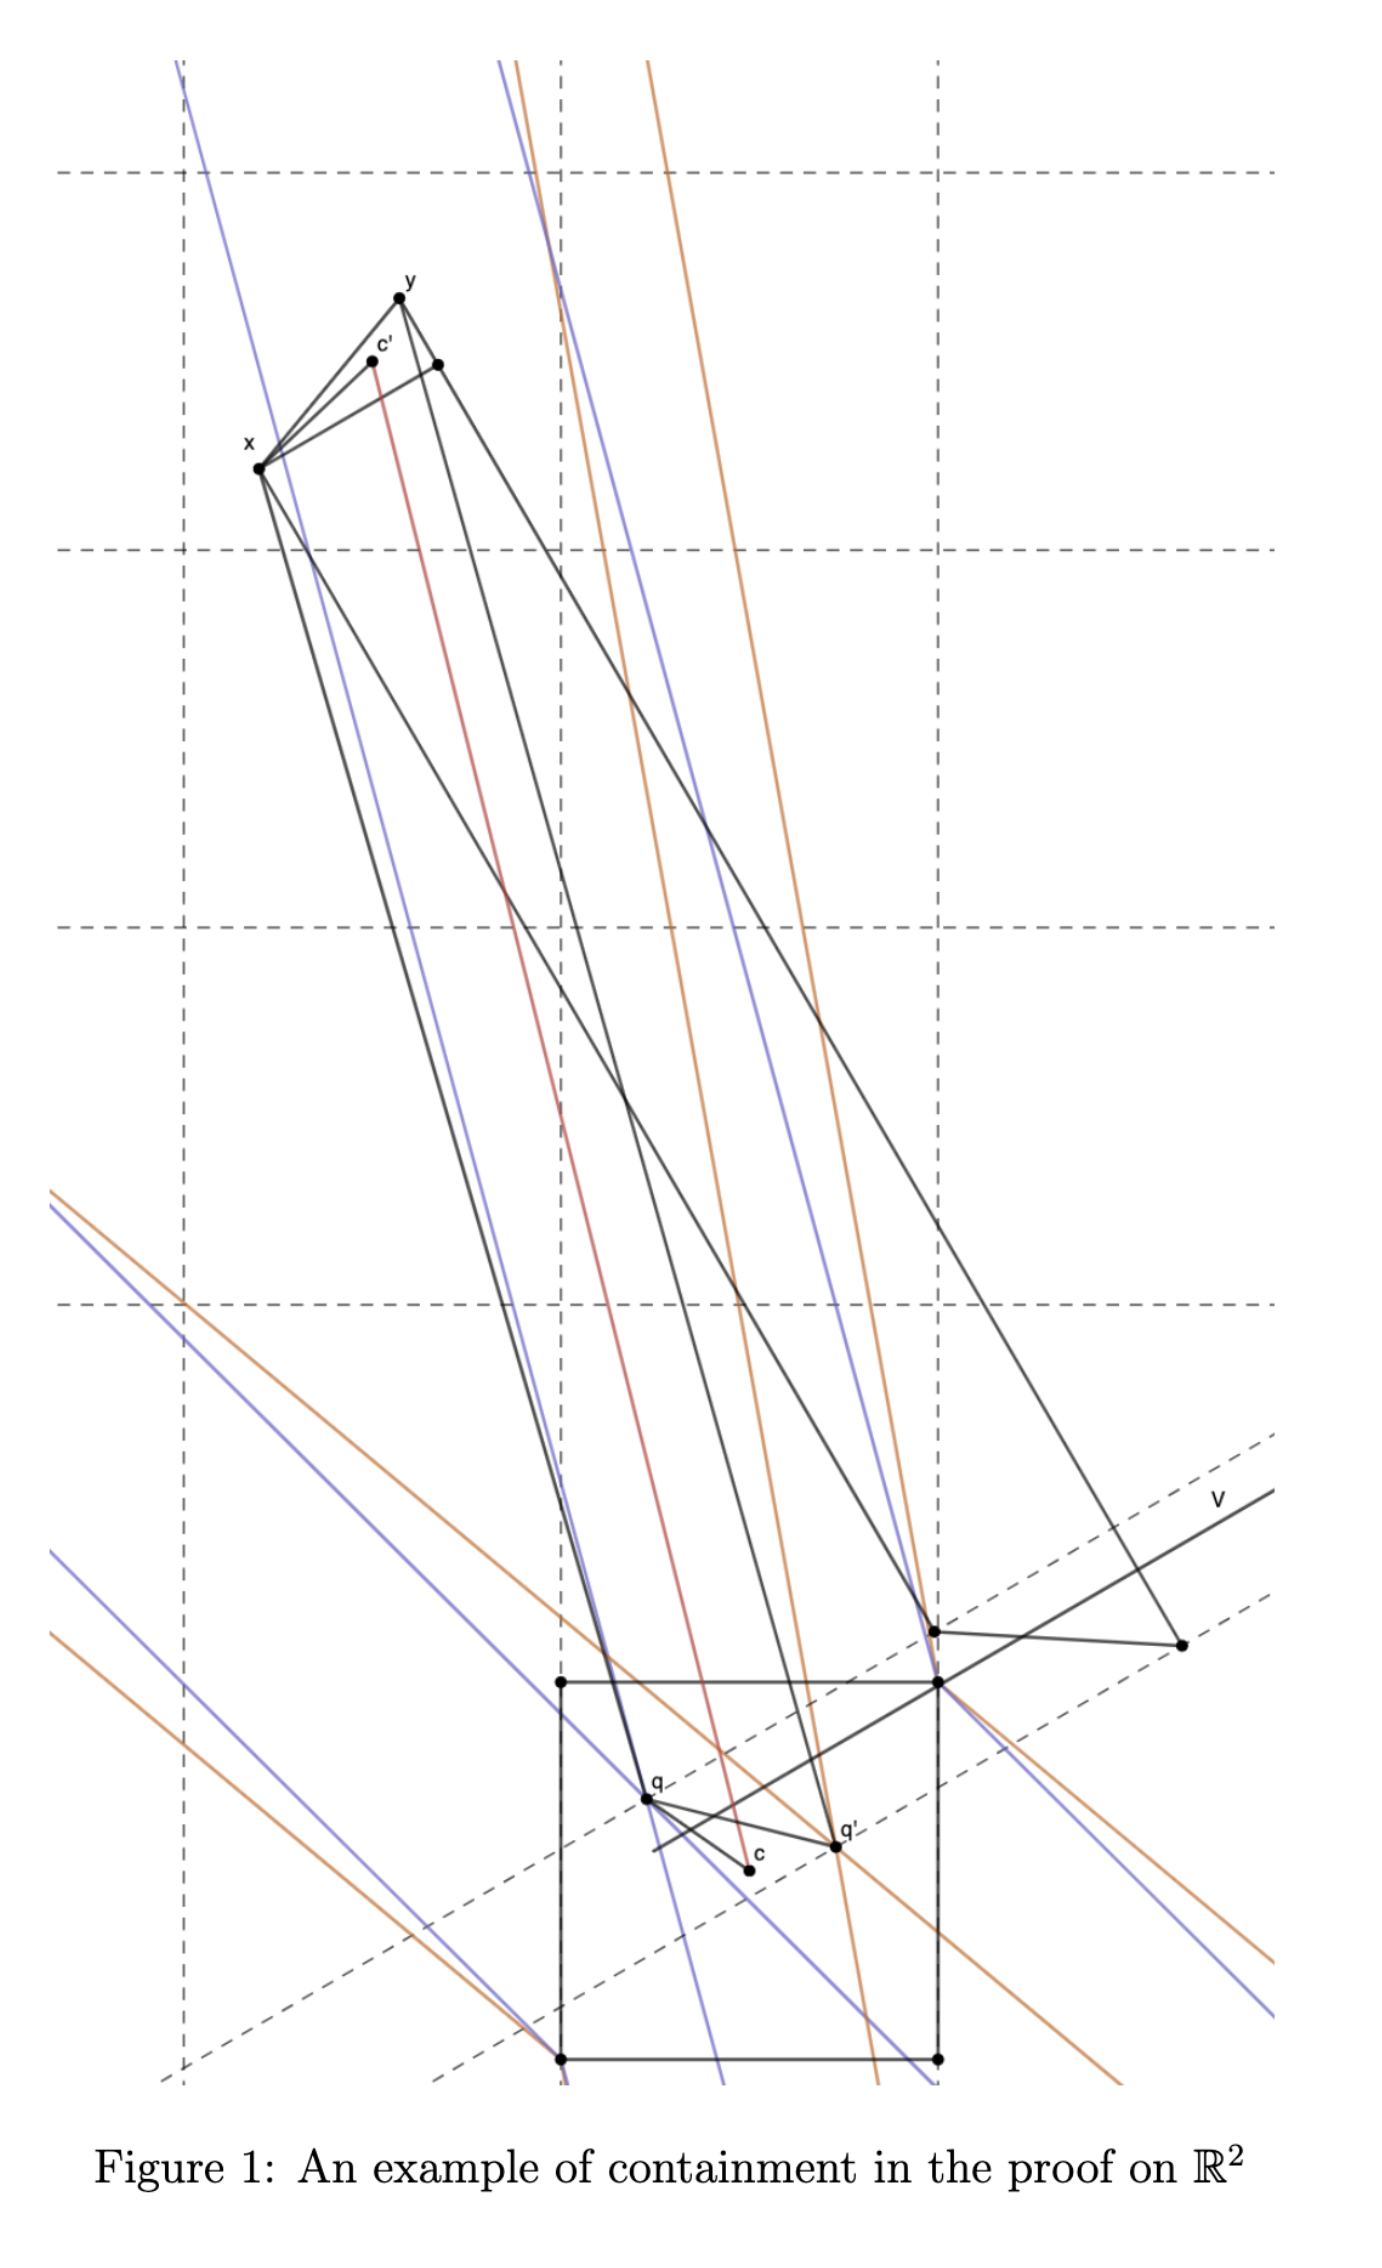
\includegraphics[width = 3in, height = 5in]{dist.png}
    \label{fig:my_label}
\end{figure}
to guarantee that $dist(y - q', V) > \alpha_2|y - q'|$ then the assumption holds. Equivalently,
\begin{equation*}
\begin{aligned}
    \alpha_1s2^{-|k|} - \sqrt{n}2^{-|k| + 1} & \geq \alpha_2|y - q'| \\
    & = \alpha_2|x-q+y-x+1-q'| \\
    & \geq \alpha_2||x - q| - |y - x| - |q - q'|| \\
    & \geq \alpha_2|s2^{-|k|} - 2^{-|k| + 1}|
\end{aligned}
\end{equation*}
And we have
\[s \geq \frac{2\sqrt{n} - 2\alpha_2}{\alpha_1 - \alpha_2}\]
Assume that the center of $Q$ is c and the center of R is c'. As $|q - c| \leq \sqrt{n}2^{-|k|-1}$ and $|x - c'|\leq \sqrt{n}2^{-|k|-1}$. Thus, 
\begin{equation*}
    \begin{aligned}
        |c - c'| & \geq ||x - q|| - |x - c'| - |q - c|| \\
        & \geq (\frac{2\sqrt{n} - 2\alpha_2}{\alpha_1 - \alpha_2} - \sqrt{n})*2^{-|k|}
    \end{aligned}
\end{equation*}
\end{proof}
\begin{lemma}
     For $\alpha_1, \alpha_2\in(0,1), \alpha_1>\alpha_2$, $V\in G(1,2)$,a cube $Q\in \mathbb{R}^2$ with side length $2^{-|k|}$, and a cube $R$ with the same side length as $Q$ s.t.
    \begin{equation}\label{eq:condition-GDBC-2}
        R\in C_B^{1,1}(Q, V, \alpha_1) \quad\text{ and }\quad R\in  C_B^{1,2}(Q, V, \alpha_2)
    \end{equation}
    let  $d\cdot \side R:=|\centerof Q-\centerof R|$ s.t.
    \begin{equation}\label{eq:tRcover2sQ-cond}
        d+\frac{\sqrt{2}}{2}\leq s \leq \sqrt{2}d-1 \quad\text{ and }\quad t \geq 2d + 2\sqrt{2}s
    \end{equation} 
    Then    
    \begin{equation}\label{eq:tRcover2sQ-conclusion}
        sQ\cap R = \emptyset \quad\text{ and }\quad R\subset 2sQ\subset tR
    \end{equation}
\end{lemma}
\begin{lemma}\label{lemma:Guarantee-Distance-contain2R-Between-2alpha}
    For $\alpha_1, \alpha_2\in(0,1), \alpha_1>\alpha_2$, $V\in G(1,2)$, a cube $Q$ in $\rr^2$ with side length $2^{-|k|}$, and a cube $R$ with the same side length as $Q$. The distance between some point in $2R$ and any point in $Q$ denoted as $s\cdot \side Q$ satisfies
    \begin{equation}\label{eq:lb4s}
        s\geq \frac{3\sqrt{2}(1+\alpha_2)}{\alpha_1-\alpha_2}
    \end{equation}
    Now
    \begin{equation}\label{eq:condition-2RinC}
        \text{if}\quad 2R\in C_B^W(Q, V, \alpha_1) \quad\text{then}\quad 2R\in  C_B^N(Q, V, \alpha_2)
    \end{equation}
\end{lemma}
\begin{lemma}
    Let $\mu$ be a doubling measure on $\mathbb{R}^2$. For $\mu$-a.e. $x \in \mathbb{R}^2$, $Q$ that contains $x$, there is an $1$-plane $V$ and an $\alpha \in(0,1)$ such that with a scaling constant $s$,
    \begin{equation}
        \lim _{Q \downarrow x} \frac{\mu\left(\mathcal{C}_\mathcal{B} (Q, V, \alpha)\right\cap 3sQ)}{\mu(3sQ)}=0
    \end{equation}
    if and only if $\mu$ is carried by Lipschitz graphs.
\end{lemma}

\begin{proof}
Fix $0 < \delta < \frac{K^{-p}}{2}$, $s \in \mathbb{N}$, 
\begin{equation}
    \frac{\mu(C_B(Q,V,\alpha)\cap 3sQ)}{\mu(3sQ)} \leq \delta \label{eq:assumption}
\end{equation}
By Lemma 6, we have \[dist(2R,Q):= s\cdot side(Q) \geq \frac{3\sqrt{2}(1 + \alpha_2)}{\alpha_1 - \alpha_2}\cdot side(Q)\]. By containment condition and doubling measure property, and 2R contains the doubling point carried by $\mu$,
\begin{equation}
    \mu(C_B(Q,V,\alpha)) \geq \mu(R) \geq K^{-p}\mu(tR) \geq K^{-p}\mu(3sQ) \label{eq:containment}
\end{equation}
By combining inequality \ref{eq:containment} and \ref{eq:assumption}, we have 
\begin{equation}
\begin{aligned}
       & K^{-p} \leq \frac{\mu(C_B(Q,V,\alpha)\cap 3sQ)}{\mu(3sQ)} \leq \delta \\
       & \rightarrow K^{-p} \leq \mu(C_B(Q,V,\alpha)\cap 3sQ) \leq \delta \mu(3sQ) \\
       & \rightarrow K^{-p} \mu(tR) \leq \mu(2R) < \delta \mu(3sQ) \\
       & \rightarrow K^{-p}\mu(3sQ) \leq\mu(2R) < \delta \mu(3sQ) \label{eq:delta}
\end{aligned}
\end{equation}
\begin{figure}
    \centering
    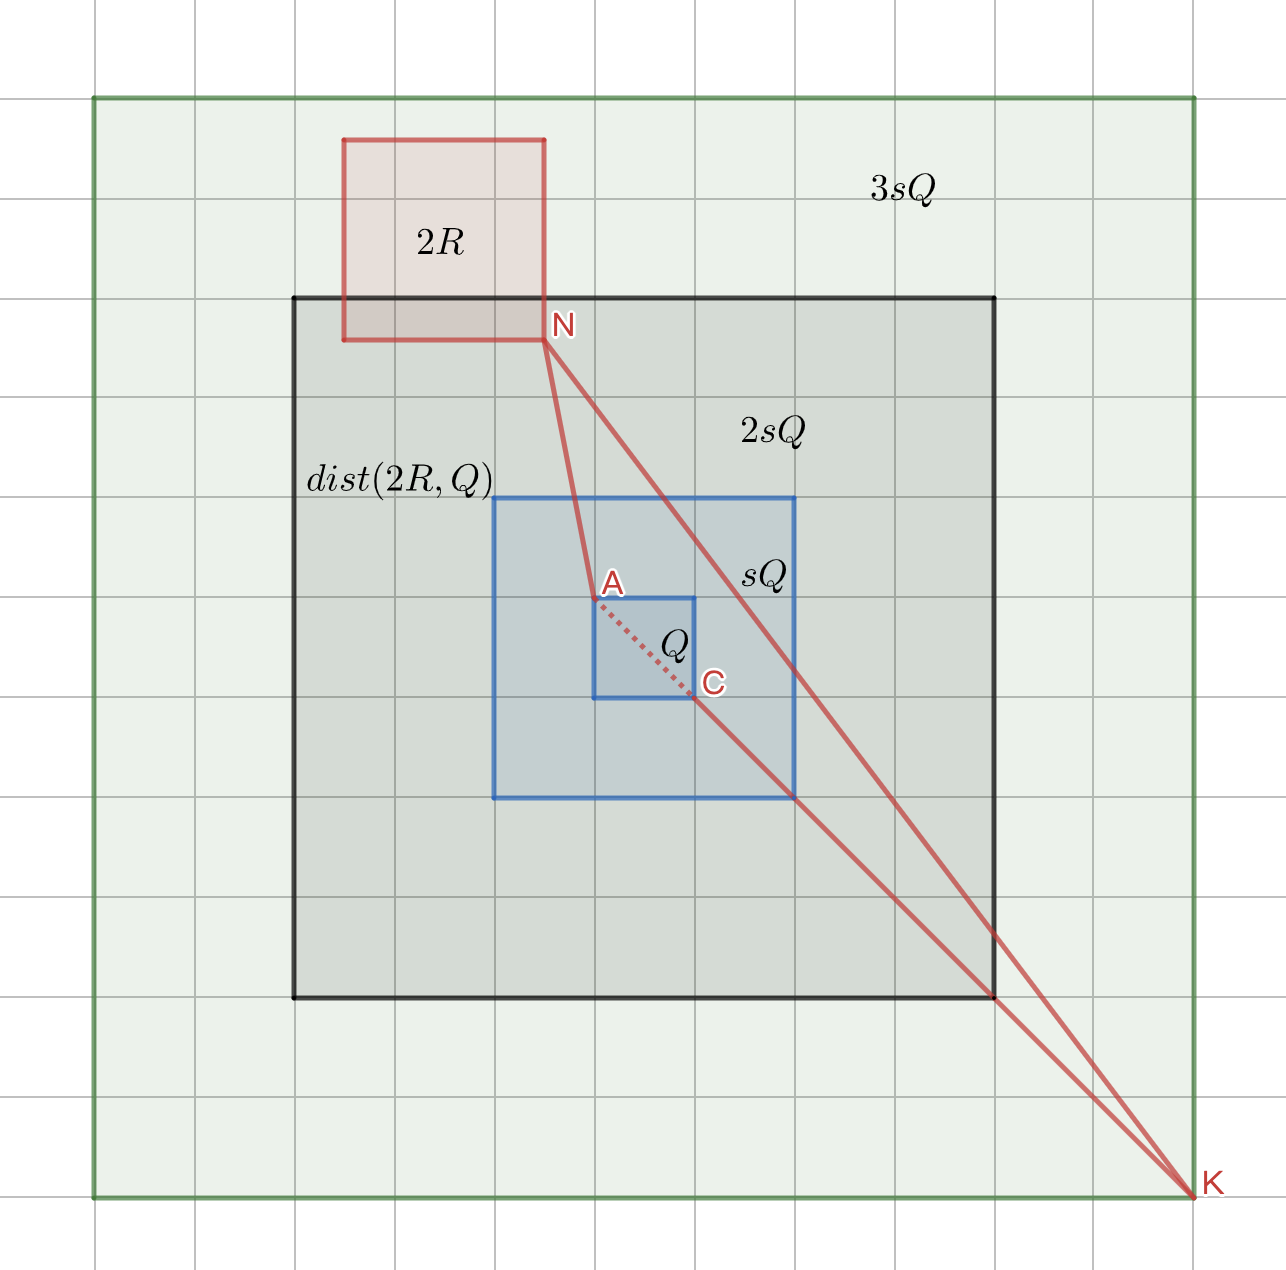
\includegraphics[width = 5in, height = 5in]{findt.png}
    \caption{An example of finding relation between R and tR}
    \label{fig:my_label}
\end{figure}
To find t, we need to determine $|N - K|$ according the figure 2, we first need to determine $|N - A|$:
\begin{equation*}
    \begin{aligned}
    |N - K| & \leq |A - K| + |N - A| \\
    & \leq (diam(Q) + |C - K|) + dist(2R,Q)\\
    & \leq (\frac{3\sqrt{2}}{2}s + \frac{\sqrt{2}}{2})side(Q) + 2s\cdot side(Q) \\
    & = \sqrt{2}(\frac{1}{2} + \frac{3}{2}s)side(Q) + 2s\cdot side(Q) \\
    & = (\frac{\sqrt{2}}{2} + \frac{3\sqrt{2}}{2}s + 2s)side(Q)
    \end{aligned}
\end{equation*}
We have that the lower and upper bound of $|N - K|$
\begin{equation*}
    \begin{aligned}
(\frac{\sqrt{2}}{2} + \frac{3\sqrt{2}}{2}s - 2s)side(Q) \leq |N - K|\leq (\frac{\sqrt{2}}{2} + \frac{3\sqrt{2}}{2}s + 2s)side(Q) \label{eq:bounds of t}
    \end{aligned}
\end{equation*}
Since 2R contains the doubling point carried by $\mu$, we have
\begin{equation*}
    \begin{aligned}
    & \mu(tR) \leq K^p\mu(2R) \\
    & \rightarrow tR \subset 2^{p}R \\
    & \rightarrow t \leq  2^{p} \\
    \end{aligned}
\end{equation*}
Thus $p \geq \log_2((\frac{\sqrt{2}}{2} + \frac{3\sqrt{2}}{2}s - 2s)side(Q))$. By inequality \ref{eq:delta}, we have $\delta\geq K^{-p}$ which contradicts to our assumption, concluding that $\mu(2R) = 0$. Therefore, as $Q \downarrow x$, we 
\end{proof}

\end{document}

% \begin{proof}
%     Since $Q,R \in \mathbb{R}^2$,by distance Lemma, we have:   
%     \begin{equation*}
%         \begin{split}
%             d \geq \left|\frac{2\sqrt{2} - 2\alpha_2}{\alpha_1-\alpha_2}-\sqrt{2}\right|
%         \end{split}
%     \end{equation*}
%     For any $q_s\in sQ, r^\prime\in R$, let $q := \centerof Q$ and $r := \centerof R$, 
%     \begin{subequations}
%         \label{s}
%         \begin{align}
%             |q - q_s| &\leq \frac{\sqrt{2}s}{2}\side Q \leq \left|\left( d-\frac{\sqrt{2}}{2}\right )\right|\side Q  \notag \\
%             &\leq ||q-r|-\frac{\sqrt{2}}{2}\side R| \notag \\
%             &\leq ||q-r| - |r - r^\prime|| \notag \\
%             &\leq |q-r^\prime| \label{eq:rtorPrime} \\ 
%             &\leq \left (d + \frac{\sqrt{2}}{2}\right)\side Q \notag \\
%             &\leq s\cdot \side Q \notag \\
%             &= \frac{1}{2}\side 2sQ\label{eq:Rin2sQ}
%         \end{align}
%     \end{subequations}
%     Equation (\ref{eq:rtorPrime}) implies that $sQ\subset B(\centerof Q, \frac{\sqrt{2}}{2}\side 2sQ)$, $r^\prime \notin B(\centerof Q, \frac{\sqrt{2}}{2}\side 2sQ)$ $\Rightarrow sQ\cap R = \emptyset$. Besides, (\ref{eq:rtorPrime}) to (\ref{eq:Rin2sQ}) implies that $R\subset B(\centerof Q, \frac{1}{2}\side 2sQ)\subset 2sQ$. For the choice of t, assume $\forall q_2\in 2sQ$, then
%     \begin{equation*}
%         |r - q_2|\leq (d+\sqrt{2}s)\side Q \leq \frac{t}{2}\side R
%     \end{equation*}
%     which implies that $2sQ \subset B(\centerof R, \frac{1}{2}\side tR)\subset tR$. Then, (\ref{eq:tRcover2sQ-conclusion}) is concluded. 
% \end{proof}



% \begin{customthm}{A}\label{thmA} 
%     Let $\mu$ be a pointwise doubling measure on $\rr^n$. For $\mu$-a.e. $x \in \rr^n$, $Q$ that contains $x$, there is an $m$-plane $V$ and an $\alpha \in(0,1)$ such that with a scaling constant $s$,
%     \begin{equation}
%         \lim _{Q \downarrow x} \frac{\mu\left(C_\calB(Q, V, \alpha)\right)}{\mu(sQ))}=0
%     \end{equation}
%     if and only if $\mu$ is carried by Lipschitz graphs.
% \end{customthm}

% We begin by establishing some geometric results that will be useful to prove Theorem $\ref{thmA}$.



% \begin{theorem}[Geometric Lemma] Let $F\subset \rr^2$, and fix $V\in G(1,2)$ and $\alpha\in(0,1)$.  If 
% 	\[F\cap \mathcal{C}_\mathcal{B}(x,V, \alpha)=\emptyset\text{ for all }x\in F\]
% 	then $F$ is contained in an $1$-Lipschitz graphs. In particular, $F\subset\Gamma$ where $\Gamma$ is a Lipschitz graph with respect to $V$ and the Lipschitz constant corresponding to $\Gamma$ is at most $1+1/(1-\alpha^2)^{1/2}$.
% 	\label{thm:geometric_lemma}
% \end{theorem}


% \begin{theorem}[Geometric Lemma] Let $F\subset \rr^2$, and fix $V\in G(1,2)$ and $\alpha\in(0,1)$.  If 
% 	\[F\cap \mathcal{C}_\mathcal{B}(x,V, \alpha)=\emptyset\text{ for all }x\in F\]
% 	then $F$ is contained in an $1$-Lipschitz graphs.  In particular, $F\subset\Gamma$ where $\Gamma$ is a Lipschitz graph with respect to $V$ and the Lipschitz constant corresponding to $\Gamma$ is at most $1+1/(1-\alpha^2)^{1/2}$.
% 	\label{thm:geometric_lemma}
% \end{theorem}